% XCircuit output "CFaccgyro.tex" for LaTeX input from CFaccgyro.ps
\def\putbox#1#2#3#4{\makebox[0in][l]{\makebox[#1][l]{}\raisebox{\baselineskip}[0in][0in]{\raisebox{#2}[0in][0in]{\scalebox{#3}{#4}}}}}
\def\rightbox#1{\makebox[0in][r]{#1}}
\def\centbox#1{\makebox[0in]{#1}}
\def\topbox#1{\raisebox{-0.60\baselineskip}[0in][0in]{#1}}
\def\midbox#1{\raisebox{-0.20\baselineskip}[0in][0in]{#1}}
   \scalebox{1}{
   \normalsize
   \parbox{4.04167in}{
   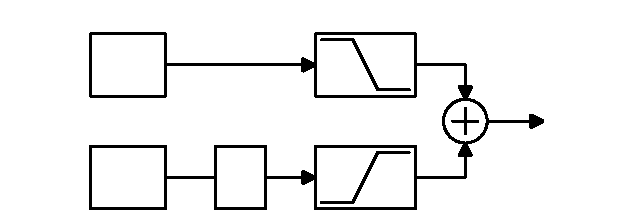
\includegraphics[scale=1]{CFaccgyro}\\
   % translate x=649 y=304 scale 0.38
   \putbox{1.60in}{0.26in}{1.20}{\centbox{\midbox{$\int$}}}%
   \putbox{2.44in}{1.26in}{1.20}{\centbox{LPF}}%
   \putbox{2.44in}{0.51in}{1.20}{\centbox{HPF}}%
   \putbox{0.85in}{1.10in}{1.20}{\centbox{\midbox{$\theta_m$}}}%
   \putbox{0.85in}{0.93in}{1.20}{\centbox{\midbox{Accel}}}%
   \putbox{0.85in}{0.18in}{1.20}{\centbox{\midbox{Gyro}}}%
   \putbox{0.85in}{0.35in}{1.20}{\centbox{\midbox{$\dot{\theta}_m$}}}%
   \putbox{3.58in}{0.79in}{1.20}{\centbox{\midbox{$\theta_e$}}}%
   } % close 'parbox'
   } % close 'scalebox'
   \vspace{-\baselineskip} % this is not necessary, but looks better
